\chapter{Dataset Shift
and Batch Normalization} \label{ch-dataset-shift}

In this chapter,
we will represent Linear Regression (LR)
as follows.
We list a dataset; i.e., a
set of tuples indexed by
the individuals $\s$
of a population $\Sigma$
such that $|\Sigma|=nsam$.
The independent variables
of the LR (i.e., $x^\s$)
are unboxed and the
 dependent variable
(a.k.a. target feature)
(i.e., $y^\s$)
is shown inside a box.
Then we show an arrow with the
superscript \enquote{LR-fit},
followed by the fit function
obtained by performing the LR.



\beq
\{(\s, x^\s =[x^\s_i],\boxed{y^\s}):\s\in \Sigma\}
\lrarr
 \haty(x)=
\alp +\sum_i x_i\beta_i
\eeq

Analogously,
we represent
Supervised Machine
 Learning (ML) as follows.


\beq
\{(\s, x^\s,\boxed{y^\s}):\s\in \Sigma\}\mlarr \haty(x)
\eeq

When doing ML, we partition  the
full population $\Sigma_{full}$
into two disjoint sets, the {\bf training set}
$\Sigma_{train}=\Sigma(\rvs=0)=\Sigma$
and the {\bf testing set}
$\Sigma_{test}=\Sigma(\rvs=1)=\Sigma^*$.
Then we do two ML fits:

\beq
\begin{array}{ll}
\text{training:}&
\{(\s, x^\s,\boxed{y^\s}):\s\in \Sigma\}\mlarr \haty(x)
\\
\text{testing:}&
\{(\s, x^\s,\boxed{y^\s}):\s\in \Sigma^*\}\mlarr \haty^*(x)
\end{array}
\eeq
Ideally, $\haty(x)$
and $\haty^*(x)$,
will be almost equal for all $x$.
Dataset shift occurs when this is not the case.
Equivalently, let

\beq
\begin{array}{lll}
P_{train}(x, y)&=P(x, y|\rvs=0) &= P(x, y)
\\
P_{test}(x, y)&=P(x, y|\rvs=1) &= P^*(x, y)
\end{array}
\eeq
We say there is a {\bf dataset shift}
if
\beq
P(x, y)\neq P^*(x, y)
\eeq

\begin{figure}[h!]
\centering
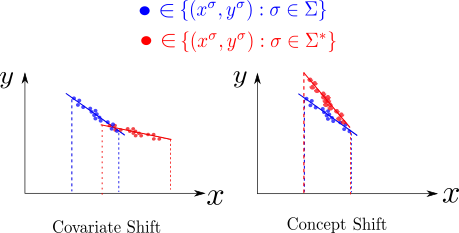
\includegraphics[width=4in]
{dataset-shift/dataset-shift.png}
\caption{For Linear Regression, 2 types
of dataset shift: covariate shift and concept shift.}
\label{fig-dataset-shift}
\end{figure}

\section{Covariate Shift}

We say there is a {\bf  covariate shift}
if (see Fig.\ref{fig-dataset-shift})

\beq
P( y|x)= P^*(y|x)
\text{ but } P(x)\neq P^*(x)
\eeq
This can be represented in terms of bnets as
follows\footnote{See
See Chapter \ref{ch-sb-removal}.}

\beq
\begin{array}{ccc}
\underbrace{\xymatrix{
\rvs=0 \ar[d]
\\
{\rvx}\ar[r]&\rvy
}}_
{\xymatrix{\\=}\xymatrix{
\rvs=0
\\
{\rvx}\ar[u]\ar[r]&\rvy
}}
&
\xymatrix{\\\neq}
&
\xymatrix{
\rvs=1\ar[d]
\\
{\rvx}\ar[r]&\rvy
}
\end{array}
\eeq


\section{Concept Shift}
We say there is a {\bf  concept shift}
if (see Fig.\ref{fig-dataset-shift})

\beq
P( y|x)\neq P^*(y|x)
\text{ but } P(x)= P^*(x)
\eeq
This can be represented in terms of bnets as
follows\footnote{See
See Chapter \ref{ch-sb-removal}.}

\beq
\begin{array}{ccc}
\underbrace{\xymatrix{
\rvs=0 \ar[rd]
\\
{\rvx}\ar[r]&\rvy
}}_
{\xymatrix{\\=}\xymatrix{
\rvs=0
\\
{\rvx}\ar[u]\ar[r]&\rvy\ar[lu]
}}
&
\xymatrix{\\\neq}
&
\xymatrix{
\rvs=1\ar[dr]
\\
{\rvx}\ar[r]&\rvy
}
\end{array}
\eeq

\section{Batch Normalization}
Batch Normalization (BN) is a technique
that is used to diminish dataset shift in Neural Nets.

Let
$h^{\lam, \s}_i$ be the output,
for individual $\s\in\Sigma$,  of the $i$th node
of layer $\lam$ of a Neural Net (NN).
Using the notation of Chapter \ref{ch-nn},

\beq
h^{\lam, \s}_i=
\cala_i^\lam(z^{\lam,\s}_i)
\eeq
where

\beq
z^{\lam,\s}_i=
\sum_j w^{\lam}_{i|j}
h^{\lam-1,\s}_j + b^{\lam}_i
\label{eq-linear-nn}
\eeq
Activation functions  $\cala^\lam_i:\RR\rarrow \RR$
for NNs
are discussed in Section \ref{sec-activation-fun}.
Suppose the population $\Sigma$ is partitioned
into disjoint batches $\Sigma^{(b)}$ for $b=1,2,\dots, B$.
Let the set of points $\{z^{\lam, \s}_i:\s\in\Sigma^{(b)}\}$
have mean $\mu^{\lam(b)}_i$
and standard deviation $\s^{\lam(b)}_i$.
For any $z^{\lam, \s}_i$ with $\s\in\Sigma$, define
the BN activation function
$\cala^\lam_{i, BN}(\cdot)$ by
\beq
\cala^\lam_{i, BN}(z^{\lam, \s}_i)=
\gamma^\lam_i
\left[
\frac{z^{\lam, \s}_i-\mu^{\lam(b)}_i}{\s^{\lam(b)}_i}
\right]+\beta^\lam_i
\quad
\text{ if }\s\in \Sigma^{(b)}
\;,
\eeq
where the real valued parameters $\gamma^\lam_i$ and $\beta^\lam_i$
are learned during the optimization process.
If node $\rvh^\lam_i$ of the NN has activation function
 $\cala^\lam_i:\RR\rarrow \RR$,
defined a new activation function $\cala^\lam_{i, new}:\RR\rarrow \RR$ by
the composition of functions
\beq
\cala^\lam_{i, new}
 =\cala^\lam_i\circ\cala^\lam_{i, BN}
\eeq
Hence, the BN activation
function
is applied after the linear transformation
Eq.(\ref{eq-linear-nn}), but before the nonlinear
transformation $\cala^\lam_i$.

Intuition on why BN diminishes dataset shift:
We discussed in Section \ref{sec-activation-fun}
how nonlinear activation functions
have a range that is smaller than their domain. Presumably, BN
helps to make the range
of the activation functions even more concentrated.
